\documentclass[11pt,a4paper,openany]{book}

\usepackage[utf8]{inputenc}
\usepackage[T1]{fontenc}
\usepackage{amsmath,amssymb,amsfonts,amsthm}
\usepackage{geometry}
\geometry{a4paper, left=2.2cm, right=2.2cm, top=2.5cm, bottom=2.5cm}

\newtheorem{theorem}{Theorem}[chapter]
\newtheorem{proposition}[theorem]{Proposition}
\newtheorem{lemma}[theorem]{Lemma}
\theoremstyle{definition}
\newtheorem{definition}[theorem]{Definition}

\usepackage{booktabs}
\usepackage{array}
\usepackage{longtable}
\usepackage{pdfpages}
\usepackage{csquotes}
\MakeOuterQuote{"}

\usepackage{xcolor}
\definecolor{mosaicblue}{RGB}{74, 128, 196}
\definecolor{mosaicpink}{RGB}{224, 102, 102}

\usepackage{tikz}
\usetikzlibrary{shapes.geometric, calc}

\usepackage[pdfusetitle, hidelinks, colorlinks=true, linkcolor=blue!70!black, citecolor=blue!70!black, urlcolor=blue!70!black]{hyperref}

\title{\textbf{An Atlas of Composition Mosaics}\\[0.4em]
\Large The Complete Dihedral Universe from $\mathbb{Z}_1$ to $\mathbb{Z}_8$}
\author{Gemma Knee \and Antigra Vitti}
\date{November 2026}

\begin{document}

\frontmatter
\maketitle

\chapter*{Preface}
\addcontentsline{toc}{chapter}{Preface}
\markboth{Preface}{Preface}

This volume presents the complete visual classification, combinatorial taxonomy, and machine-readable relational inventory of composition mosaics across the circular rings $\mathbb{Z}_1$ through $\mathbb{Z}_8$.

As the third monograph in our coffee-table trilogy on the combinatorial geometry of circular lattices---standing alongside \emph{The Polygonal Burnsidean: An Atlas of Inscribed Polygons from $\mathbb{Z}_1$ to $\mathbb{Z}_{16}$}~\cite{KneeVitti2026poly} and \emph{Hexadecality: The Sixteen-Lattice Universe}~\cite{KneeVitti2026hex}---this atlas unifies the full progression of cyclic lattices from the elementary monad to the rich octagonal universe:
\begin{itemize}
    \item Across the first eight rings $\mathbb{Z}_1$ through $\mathbb{Z}_8$, the combinatorial universe generates exactly $5{,}295$ set partitions, governed by the initial segment of the Bell numbers $B_1 = 1, B_2 = 2, B_3 = 5, B_4 = 15, B_5 = 52, B_6 = 203, B_7 = 877$, and $B_8 = 4{,}140$.
    \item Under the physical symmetries of the respective dihedral groups $D_n$, these $5{,}295$ partitions collapse into exactly $\mathbf{509}$ non-equivalent dihedral composition mosaics, realising the initial terms of sequence OEIS A084708:
    \begin{equation*}
    1, \; 2, \; 3, \; 7, \; 12, \; 37, \; 93, \; 354 \quad \implies \quad \sum_{n=1}^8 M_n = 509
    \end{equation*}
    \item The eight lattices capture the full structural spectrum of cyclic geometry: the trivial monad $\mathbb{Z}_1$; the reflexive dyad $\mathbb{Z}_2$; the odd prime rings $\mathbb{Z}_3, \mathbb{Z}_5, \mathbb{Z}_7$; the composite square lattice $\mathbb{Z}_4$; the composite hexagonal lattice $\mathbb{Z}_6$ where scalene triangles and chiral enantiomorphic blocks first emerge into the geometric universe; and the cubic power-of-two lattice $\mathbb{Z}_8$, which hosts the unique cyclic Skolem difference sequence of order $4$.
    \item Through the two-vertex domino inflation functor, the 8-vertex Skolem partition acts as the seed for higher-order affine macro-orbits on the 16-cycle $\mathbb{Z}_{16}$, creating an explicit mathematical bridge connecting all three volumes of the trilogy.
\end{itemize}

\section*{Cartographic Conventions and Visual Aesthetics}

Each mosaic in this atlas is presented in pure geometric form. The partition blocks appear as shaded convex inscribed polygons, metric chords, and vertex pips within the circular frame of the regular $n$-gon, unencumbered by peripheral coordinate clutter:
\begin{itemize}
    \item \textbf{Achiral Blocks (Blue)}: Inscribed polygons possessing an internal axis of bilateral reflection symmetry across the cyclic lattice.
    \item \textbf{Chiral Blocks (Pink)}: Scalene polygons that lack reflectional symmetry, existing as one half of an enantiomorphic pair.
\end{itemize}

The complete visual catalogue in Chapter~\ref{chap:visual-atlas} displays all $509$ configurations arranged in a strict taxonomic sequence across ten high-density vector plates. All accompanying analytical invariants---dihedral orbit sizes $|\mathcal{O}|$, stabiliser subgroups, Fa\`a di Bruno partition multiplicities, chord dispersion energies, polygon profiles, and relational manifests linking directly into \emph{The Polygonal Burnsidean}---are systematically catalogued in Chapter~\ref{chap:canonical-taxonomy} and in the companion machine-readable open datasets.

\bigskip
\begin{flushright}
\textbf{Gemma Knee} \qquad \textbf{Antigra Vitti} \\
\emph{Newcastle upon Tyne} \\
\emph{November 2026}
\end{flushright}


\tableofcontents

\mainmatter

\chapter{Lattice Geometry and Combinatorial Invariants}
\label{chap:lattice-architecture}

\section{Circular Lattices and Dihedral Symmetries}

Let $\mathbb{Z}_n = \{0, 1, \dots, n-1\}$ denote the cyclic ring of integers modulo $n$, geometrically embedded as the vertices of a regular $n$-gon inscribed in the unit circle and oriented clockwise with vertex $0$ positioned at the zenith. 

The physical isometries of the polygon constitute the dihedral group $D_n$. For $n \ge 3$, $D_n$ has order $2n$ with presentation:
\begin{equation}
D_n = \langle \rho, \tau \mid \rho^n = \tau^2 = 1, \; \tau \rho \tau = \rho^{-1} \rangle
\end{equation}
generated by the clockwise unit rotation $\rho \colon x \mapsto x + 1 \pmod n$ and the vertical bilateral chord reflection $\tau \colon x \mapsto -x \equiv n - x \pmod n$. For the degenerate small rings, the isometry groups coincide with the physical symmetries:
\begin{equation}
D_1 = \{1\} \; (|D_1| = 1), \qquad D_2 = \langle \rho \mid \rho^2 = 1 \rangle \cong C_2 \; (|D_2| = 2)
\end{equation}
where on two vertices the single reflection $x \mapsto 1 - x \pmod 2$ acts identically to the transposition rotation $\rho$. For any $n \ge 1$, the reflections in $D_n$ are precisely the involutions $x \mapsto b - x \pmod n$ for $b \in \mathbb{Z}_n$.

A \textbf{composition mosaic} $\mathcal{M}$ on $\mathbb{Z}_n$ is a set partition of the $n$ vertices into $s$ non-empty, pairwise disjoint blocks:
\begin{equation}
\mathcal{M} = \{B_1, B_2, \dots, B_s\}, \quad \bigcup_{j=1}^s B_j = \mathbb{Z}_n, \quad B_i \cap B_j = \emptyset \; (i \neq j)
\end{equation}
Each constituent block $B_j \subset \mathbb{Z}_n$ of cardinality $d_j = |B_j| \ge 1$ forms an inscribed polygon in the lattice:
\begin{itemize}
    \item A \textbf{unigon} ($d_j = 1$), visualised as a central circular pip on vertex $v \in \mathbb{Z}_n$.
    \item A \textbf{digon} ($d_j = 2$), visualised as a straight metric chord connecting the vertex pair.
    \item An \textbf{inscribed polygon} ($d_j \ge 3$), visualised as a shaded convex polygonal tile bounded by circular perimeter chords.
\end{itemize}

\section{The Graded Stratification of Set Partitions}

Across the full combinatorial universe, the total number of set partitions of an $n$-element set is given by the $n$-th Bell number $B_n$:
\begin{equation}
B_n = \sum_{s=1}^n \genfrac{\{}{\}}{0pt}{}{n}{s}
\end{equation}
where $\genfrac{\{}{\}}{0pt}{}{n}{s}$ denotes the Stirling numbers of the second kind, enumerating set partitions into exactly $s$ blocks. 

The space of partitions further stratifies according to the unordered multiset of block sizes, termed the \textbf{partition shape} $\lambda = (\lambda_1, \dots, \lambda_s) \vdash n$, where $\lambda_1 \ge \lambda_2 \ge \dots \ge \lambda_s \ge 1$ and $\sum_{j=1}^s \lambda_j = n$. For each shape $\lambda \vdash n$, the exact number of set partitions is governed by the Fa\`a di Bruno multinomial formula:
\begin{equation}
p_\lambda = \frac{n!}{\prod_{i=1}^n (i!)^{c_i} \, c_i!}
\end{equation}
where $c_i = c_i(\lambda)$ is the multiplicity of parts of size $i$ in $\lambda$.

Across the first eight rings $\mathbb{Z}_1$ through $\mathbb{Z}_8$, the Bell numbers grow rapidly:
\begin{equation*}
B_1 = 1, \quad B_2 = 2, \quad B_3 = 5, \quad B_4 = 15, \quad B_5 = 52, \quad B_6 = 203, \quad B_7 = 877, \quad B_8 = 4{,}140
\end{equation*}
yielding a total combinatorial universe of exactly $5{,}295$ set partitions.

\section{The Dihedral Orbit Inventory and Burnsidean Enumeration}

The dihedral group $D_n$ acts on the space of set partitions $\mathcal{P}(\mathbb{Z}_n)$ by permuting the underlying coordinates:
\begin{equation}
g \cdot \{B_1, \dots, B_s\} = \{g(B_1), \dots, g(B_s)\} \quad (g \in D_n)
\end{equation}
Because the group action is an isometry, it preserves the part count $s$, the individual block cardinalities $|B_j|$, and the partition shape $\lambda \vdash n$. The set partitions of shape $\lambda$ decompose into disjoint $D_n$-orbits:
\begin{equation}
\mathcal{O}(\mathcal{M}) = \{g \cdot \mathcal{M} \mid g \in D_n\}
\end{equation}

By the Orbit-Stabiliser Theorem, the length of any orbit $|\mathcal{O}| = k$ must divide the group order $|D_n|$. The stabiliser subgroup $\operatorname{Stab}_{D_n}(\mathcal{M})$ has order $|D_n| / k$.

Summing the orbit multiplicities $a_{k,\lambda}$ yields the graded bivariate orbit polynomial $P_n(\mathbf{z}, \omega)$:
\begin{equation}
P_n(\mathbf{z}, \omega) = \sum_{\lambda \vdash n} Q_\lambda(\omega) \mathbf{z}^\lambda = \sum_{\lambda \vdash n} \left( \sum_{k \mid |D_n|} a_{k,\lambda} \omega^k \right) \mathbf{z}^\lambda
\end{equation}
Evaluating this polynomial at $\omega = 1$ recovers the total count $M_n$ of non-equivalent dihedral composition mosaics on $\mathbb{Z}_n$. Table~\ref{tab:census-z1-z8} presents the consolidated inventory across the eight lattices, recovering the initial terms of OEIS sequence A084708 and establishing the grand total of $\mathbf{509}$ non-equivalent dihedral composition mosaics.

% Auto-generated by generate_multilattice_atlas.py
\begin{table}[htbp]
\centering
\small
\caption{\label{tab:census-z1-z8}Consolidated Dihedral Mosaic Census from $\mathbb{Z}_1$ to $\mathbb{Z}_8$ (OEIS A084708)}
\begin{tabular}{c r r r r l}
\toprule
Ring $\mathbb{Z}_n$ & $|D_n|$ & Partitions $B_n$ & Shapes & Dihedral Mosaics & Orbit Size Decomposition $\sum a_k \omega^k$ \\
\midrule
$\mathbb{Z}_1$ & 1 & 1 & 1 & \textbf{1} & $1\omega^{1}$ \\
$\mathbb{Z}_2$ & 2 & 2 & 2 & \textbf{2} & $2\omega^{1}$ \\
$\mathbb{Z}_3$ & 6 & 5 & 3 & \textbf{3} & $2\omega^{1} + 1\omega^{3}$ \\
$\mathbb{Z}_4$ & 8 & 15 & 5 & \textbf{7} & $3\omega^{1} + 2\omega^{2} + 2\omega^{4}$ \\
$\mathbb{Z}_5$ & 10 & 52 & 7 & \textbf{12} & $2\omega^{1} + 10\omega^{5}$ \\
$\mathbb{Z}_6$ & 12 & 203 & 11 & \textbf{37} & $4\omega^{1} + 2\omega^{2} + 9\omega^{3} + 16\omega^{6} + 6\omega^{12}$ \\
$\mathbb{Z}_7$ & 14 & 877 & 15 & \textbf{93} & $2\omega^{1} + 57\omega^{7} + 34\omega^{14}$ \\
$\mathbb{Z}_8$ & 16 & 4,140 & 22 & \textbf{354} & $4\omega^{1} + 6\omega^{2} + 27\omega^{4} + 132\omega^{8} + 185\omega^{16}$ \\
\midrule\midrule
\textbf{Total} & --- & \textbf{5,295} & \textbf{66} & \textbf{509} & --- \\
\bottomrule
\end{tabular}
\end{table}


\section{The Bilateral Symmetry Classification}

Every individual block $B \subset \mathbb{Z}_n$ within a mosaic possesses an internal circular stride composition $(s_1, \dots, s_d)$ satisfying $\sum_{i=1}^d s_i = n$. A block is defined as \textbf{bilaterally symmetric} (or achiral) if it is invariant under at least one reflection $x \mapsto b - x \pmod n$ of the circular lattice. 

Under this classification:
\begin{itemize}
    \item \textbf{Achiral Blocks (Blue)}: Inscribed polygons possessing an internal reflection axis. On any lattice $\mathbb{Z}_n$, every unigon ($d=1$), every digon chord ($d=2$), and every regular or isosceles polygon is strictly achiral.
    \item \textbf{Chiral Blocks (Pink)}: Scalene polygons whose circular stride sequence is not invariant under cyclic reversal.
\end{itemize}

\begin{theorem}[Emergence of Block Chirality]
On the circular lattices $\mathbb{Z}_n$, all constituent blocks of all set partitions are strictly achiral for $n \le 5$. Chiral blocks emerge if and only if $n \ge 6$ and block cardinality $d \ge 3$. The minimal chiral block is the scalene triangle of circular strides $(1, 2, 3)$ on the hexagonal lattice $\mathbb{Z}_6$.
\end{theorem}

\begin{proof}
For block size $d \in \{1, 2\}$, any unigon is trivially self-symmetric, and any digon $\{u, v\}$ is invariant under the reflection through the perpendicular bisector of the chord $u \leftrightarrow v$, which is a valid lattice reflection for every $n$. 

For $d = 3$, an inscribed triangle with stride composition $(s_1, s_2, s_3)$ is chiral if and only if the strides are pairwise distinct (scalene). The minimal sum of three distinct positive integers is $1 + 2 + 3 = 6$. Hence no chiral triangle can exist for $n < 6$. For $n = 6$, the unique integer partition into three distinct parts is $1 + 2 + 3 = 6$, realised by the block $\{0, 1, 3\}$ with strides $(1, 2, 3)$. Under reflection $x \mapsto b - x \pmod 6$, the stride sequence reverses to $(3, 2, 1) \equiv (1, 3, 2) \not\equiv (1, 2, 3)$ under cyclic shifts. Hence $\{0, 1, 3\}$ possesses no internal reflection symmetry and is chiral.
\end{proof}

A mosaic $\mathcal{M}$ is characterised by its \textbf{chirality signature}, recording the binary achiral/chiral character of its sorted constituent blocks (e.g. $[ssss]$ for an all-symmetric mosaic, $[sscc]$ for a mosaic containing two symmetric and two chiral blocks). In the visual atlas, chiral blocks appear in distinctive rose-pink shading, highlighting the subtle symmetry-breaking phenomena that first emerge on $\mathbb{Z}_6$.

\section{The Singleton Shattering Duality}

A foundational structural property uniting all cyclic lattices is the \textbf{Singleton Shattering Duality}~\cite{Joyal1981,Kerber1999}. For any partition shape $\lambda = (b_1, \dots, b_{s-1}, a) \vdash n$ possessing a distinguished block of size $a \ge 2$, shattering this block into $a$ individual singleton vertices ($a \to 1^a$) forms an equivariant bijection between point stabilisers.

Consequently, the orbit polynomial is identically preserved under singleton replacement:
\begin{equation}
Q_{(b_1, \dots, b_{s-1}, a)}(\omega) \equiv Q_{(b_1, \dots, b_{s-1}, 1^a)}(\omega)
\end{equation}
This duality creates exact isomorphisms between coarse and fine partition shapes across every ring:
\begin{align}
\text{On } \mathbb{Z}_4\colon \quad z_4 &\longleftrightarrow z_1^4 && (1\omega^1) \\
\text{On } \mathbb{Z}_5\colon \quad z_5 &\longleftrightarrow z_1^5 && (1\omega^1) \\
\text{On } \mathbb{Z}_6\colon \quad z_6 &\longleftrightarrow z_1^6 && (1\omega^1) \\
z_2 z_4 &\longleftrightarrow z_1^4 z_2 && (2\omega^6 + \omega^2) \\
\text{On } \mathbb{Z}_8\colon \quad z_8 &\longleftrightarrow z_1^8 && (1\omega^1) \\
z_2 z_6 &\longleftrightarrow z_1^6 z_2 && (3\omega^8 + \omega^4) \\
z_3 z_5 &\longleftrightarrow z_1^5 z_3 && (2\omega^{16} + 3\omega^8) \\
z_2^2 z_4 &\longleftrightarrow z_1^4 z_2^2 && (7\omega^{16} + 10\omega^8 + 4\omega^4 + \omega^2)
\end{align}

\section{Circular Chord Energy}

The spatial dispersion of a composition mosaic $\mathcal{M} = \{B_1, \dots, B_s\}$ on $\mathbb{Z}_n$ is quantified by its \textbf{chord dispersion energy} $E(\mathcal{M})$:
\begin{equation}
E(\mathcal{M}) = \sum_{B \in \mathcal{M}} \sum_{u < v \in B} \min(|u - v|, n - |u - v|)^2
\end{equation}
defined as the sum of squared circular shortest-path distances across all internal edges of every constituent block. 

Configurations whose vertices are closely clustered span small perimeter strides and exhibit low energy, whereas configurations whose vertices are diametrically distributed across the lattice maximise chord dispersion. Within any given partition shape, chord energy provides a natural geometric gradient for canonical ordering.

\section{The Cyclic Skolem Structure on \texorpdfstring{$\mathbb{Z}_8$}{Z8} and Domino Inflation}

On the eight-vertex ring $\mathbb{Z}_8$, the partition shape $z_2^4$ divides the lattice into four disjoint 2-vertex digons. Across the $17$ dihedral orbits of shape $z_2^4$, exactly one orbit achieves the minimal difference-covering configuration:
\begin{equation}
\mathcal{M}_{\text{Skolem}} = \{\{0, 1\}, \{4, 6\}, \{2, 5\}, \{3, 7\}\} \equiv \texttt{/01/25/37/46/}
\end{equation}
The four constituent chords span circular distances:
\begin{equation}
\text{dist}(0, 1) = 1, \quad \text{dist}(4, 6) = 2, \quad \text{dist}(2, 5) = 3, \quad \text{dist}(3, 7) = 4
\end{equation}
covering each non-zero circular distance $\{1, 2, 3, 4\}$ on $\mathbb{Z}_8$ exactly once. 

This configuration is the celebrated \textbf{unique cyclic Skolem sequence of order 4 on $\mathbb{Z}_8$}~\cite{Skolem1957}, corresponding to the canonical circular word $(1, 1, 3, 4, 2, 3, 2, 4)$. In our canonical inventory, it is catalogued as local orbit 227 of $\mathbb{Z}_8$ (global ID \textbf{382}).

Under the two-vertex domino inflation functor $\mathcal{I}_{\text{domino}} \colon k \mapsto \{2k - 1, 2k\} \pmod{16}$, each vertex of $\mathbb{Z}_8$ expands into a contiguous pair of adjacent vertices on the 16-cycle $\mathbb{Z}_{16}$. Under this inflation, $\mathcal{M}_{\text{Skolem}}$ maps directly to the four-chord skeleton underlying the cyclic Skolem affine macro-orbit (catalogued as macro-orbit $T00646$ in \emph{Hexadecality}). The octonary universe thus provides the fundamental seed for affine macro-orbits on higher-order power-of-two lattices.

\chapter{The Canonical Dihedral Catalogue}
\label{chap:canonical-taxonomy}

\section{Taxonomic Ordering Principles}

The $509$ dihedral composition mosaics across $\mathbb{Z}_1$ through $\mathbb{Z}_8$ are organised according to a four-tier hierarchical classification:

\begin{enumerate}
    \item \textbf{Tier 1 (Lattice Ring Progression)}: Mosaics are stratified primarily by the underlying circular lattice order $n \in \{1, 2, \dots, 8\}$.
    
    \item \textbf{Tier 2 (Part-Count Stratification)}: Within each ring $\mathbb{Z}_n$, mosaics are stratified by the number of constituent blocks $s = \ell(\lambda) \in \{1, \dots, n\}$, corresponding to the Stirling numbers of the second kind.
    
    \item \textbf{Tier 3 (Lexicographical Shape Ordering)}: Within each stratum $s$, individual partition shapes $\lambda = (\lambda_1, \dots, \lambda_s) \vdash n$ follow standard lexicographical order:
    \begin{equation}
    (n) \prec (n-1, 1) \prec (n-2, 2) \prec \dots \prec (2, 1^{n-2}) \prec (1^n)
    \end{equation}
    
    \item \textbf{Tier 4 (Intra-Shape Ordering)}: Within each individual shape $\lambda$, non-equivalent dihedral orbits are ordered deterministically by:
    \begin{itemize}
        \item \textbf{Symmetric Block Count ($s_{\text{sym}}$ Descending)}: Fully achiral configurations precede mixed configurations, which precede chiral configurations.
        \item \textbf{Chord Energy ($E$ Descending)}: Mosaics spanning longer circular distances precede localized configurations:
        \begin{equation}
        E(\mathcal{M}) = \sum_{B \in \mathcal{M}} \sum_{u < v \in B} \min(|u - v|, n - |u - v|)^2
        \end{equation}
        \item \textbf{Canonical Representative String}: Deterministic tie-breaking is governed by the lexicographical order of the hexadecimal slash-delimited partition notation.
    \end{itemize}
\end{enumerate}

Every orbit is assigned both a global integer identifier $1 \dots 509$ spanning the full octonary universe and a local ring identifier $1 \dots M_n$, directly matching its appearance in the visual plates of Chapter~\ref{chap:visual-atlas}.

\section{Stratified Partition Shape Inventory}

Table~\ref{tab:shape-census-z1-z8} details the complete partition shape inventory across all eight rings $\mathbb{Z}_1$ through $\mathbb{Z}_8$, recording the number of set partitions $p_\lambda$, the number of non-equivalent dihedral mosaics, the shape monomial $\mathbf{z}^\lambda$, and the bivariate orbit polynomial $Q_\lambda(\omega)$.

% Auto-generated by generate_multilattice_atlas.py
\begin{longtable}{r r l l}
\caption{\label{tab:shape-census-z1-z8}Stratified Partition Shape Inventory for $\mathbb{Z}_1$ through $\mathbb{Z}_8$}\\
\toprule
Partitions $\#p$ & Mosaics $\#o$ & Partition Shape Monomial $\mathbf{z}^\lambda$ & Orbit Polynomial $Q_\lambda(\omega)$ \\
\midrule
\endfirsthead
\caption[]{Stratified Partition Shape Inventory (continued)}\\
\toprule
Partitions $\#p$ & Mosaics $\#o$ & Partition Shape Monomial $\mathbf{z}^\lambda$ & Orbit Polynomial $Q_\lambda(\omega)$ \\
\midrule
\endhead
\bottomrule
\endfoot
\midrule
\multicolumn{4}{c}{\textbf{Ring $\mathbb{Z}_1$} ($|D_1|=1$, $B_1=1$, 1 Mosaics)} \\
\midrule
1 & 1 & $z_1$ & $1\omega^{1}$ \\
\midrule
\multicolumn{4}{c}{\textbf{Ring $\mathbb{Z}_2$} ($|D_2|=2$, $B_2=2$, 2 Mosaics)} \\
\midrule
1 & 1 & $z_2$ & $1\omega^{1}$ \\
1 & 1 & $z_1^2$ & $1\omega^{1}$ \\
\midrule
\multicolumn{4}{c}{\textbf{Ring $\mathbb{Z}_3$} ($|D_3|=6$, $B_3=5$, 3 Mosaics)} \\
\midrule
1 & 1 & $z_3$ & $1\omega^{1}$ \\
3 & 1 & $z_2 z_1$ & $1\omega^{3}$ \\
1 & 1 & $z_1^3$ & $1\omega^{1}$ \\
\midrule
\multicolumn{4}{c}{\textbf{Ring $\mathbb{Z}_4$} ($|D_4|=8$, $B_4=15$, 7 Mosaics)} \\
\midrule
1 & 1 & $z_4$ & $1\omega^{1}$ \\
4 & 1 & $z_3 z_1$ & $1\omega^{4}$ \\
3 & 2 & $z_2^2$ & $1\omega^{1} + 1\omega^{2}$ \\
6 & 2 & $z_2 z_1^2$ & $1\omega^{2} + 1\omega^{4}$ \\
1 & 1 & $z_1^4$ & $1\omega^{1}$ \\
\midrule
\multicolumn{4}{c}{\textbf{Ring $\mathbb{Z}_5$} ($|D_5|=10$, $B_5=52$, 12 Mosaics)} \\
\midrule
1 & 1 & $z_5$ & $1\omega^{1}$ \\
5 & 1 & $z_4 z_1$ & $1\omega^{5}$ \\
10 & 2 & $z_3 z_2$ & $2\omega^{5}$ \\
10 & 2 & $z_3 z_1^2$ & $2\omega^{5}$ \\
15 & 3 & $z_2^2 z_1$ & $3\omega^{5}$ \\
10 & 2 & $z_2 z_1^3$ & $2\omega^{5}$ \\
1 & 1 & $z_1^5$ & $1\omega^{1}$ \\
\midrule
\multicolumn{4}{c}{\textbf{Ring $\mathbb{Z}_6$} ($|D_6|=12$, $B_6=203$, 37 Mosaics)} \\
\midrule
1 & 1 & $z_6$ & $1\omega^{1}$ \\
6 & 1 & $z_5 z_1$ & $1\omega^{6}$ \\
15 & 3 & $z_4 z_2$ & $1\omega^{3} + 2\omega^{6}$ \\
10 & 3 & $z_3^2$ & $1\omega^{1} + 1\omega^{3} + 1\omega^{6}$ \\
15 & 3 & $z_4 z_1^2$ & $1\omega^{3} + 2\omega^{6}$ \\
60 & 6 & $z_3 z_2 z_1$ & $2\omega^{6} + 4\omega^{12}$ \\
15 & 5 & $z_2^3$ & $1\omega^{1} + 1\omega^{2} + 2\omega^{3} + 1\omega^{6}$ \\
20 & 3 & $z_3 z_1^3$ & $1\omega^{2} + 1\omega^{6} + 1\omega^{12}$ \\
45 & 8 & $z_2^2 z_1^2$ & $3\omega^{3} + 4\omega^{6} + 1\omega^{12}$ \\
15 & 3 & $z_2 z_1^4$ & $1\omega^{3} + 2\omega^{6}$ \\
1 & 1 & $z_1^6$ & $1\omega^{1}$ \\
\midrule
\multicolumn{4}{c}{\textbf{Ring $\mathbb{Z}_7$} ($|D_7|=14$, $B_7=877$, 93 Mosaics)} \\
\midrule
1 & 1 & $z_7$ & $1\omega^{1}$ \\
7 & 1 & $z_6 z_1$ & $1\omega^{7}$ \\
21 & 3 & $z_5 z_2$ & $3\omega^{7}$ \\
35 & 4 & $z_4 z_3$ & $3\omega^{7} + 1\omega^{14}$ \\
21 & 3 & $z_5 z_1^2$ & $3\omega^{7}$ \\
105 & 9 & $z_4 z_2 z_1$ & $3\omega^{7} + 6\omega^{14}$ \\
70 & 7 & $z_3^2 z_1$ & $4\omega^{7} + 3\omega^{14}$ \\
105 & 12 & $z_3 z_2^2$ & $9\omega^{7} + 3\omega^{14}$ \\
35 & 4 & $z_4 z_1^3$ & $3\omega^{7} + 1\omega^{14}$ \\
210 & 18 & $z_3 z_2 z_1^2$ & $6\omega^{7} + 12\omega^{14}$ \\
105 & 11 & $z_2^3 z_1$ & $7\omega^{7} + 4\omega^{14}$ \\
35 & 4 & $z_3 z_1^4$ & $3\omega^{7} + 1\omega^{14}$ \\
105 & 12 & $z_2^2 z_1^3$ & $9\omega^{7} + 3\omega^{14}$ \\
21 & 3 & $z_2 z_1^5$ & $3\omega^{7}$ \\
1 & 1 & $z_1^7$ & $1\omega^{1}$ \\
\midrule
\multicolumn{4}{c}{\textbf{Ring $\mathbb{Z}_8$} ($|D_8|=16$, $B_8=4140$, 354 Mosaics)} \\
\midrule
1 & 1 & $z_8$ & $1\omega^{1}$ \\
8 & 1 & $z_7 z_1$ & $1\omega^{8}$ \\
28 & 4 & $z_6 z_2$ & $1\omega^{4} + 3\omega^{8}$ \\
56 & 5 & $z_5 z_3$ & $3\omega^{8} + 2\omega^{16}$ \\
35 & 7 & $z_4^2$ & $1\omega^{1} + 1\omega^{2} + 2\omega^{4} + 3\omega^{8}$ \\
28 & 4 & $z_6 z_1^2$ & $1\omega^{4} + 3\omega^{8}$ \\
168 & 12 & $z_5 z_2 z_1$ & $3\omega^{8} + 9\omega^{16}$ \\
280 & 19 & $z_4 z_3 z_1$ & $3\omega^{8} + 16\omega^{16}$ \\
210 & 22 & $z_4 z_2^2$ & $1\omega^{2} + 4\omega^{4} + 10\omega^{8} + 7\omega^{16}$ \\
280 & 25 & $z_3^2 z_2$ & $2\omega^{4} + 12\omega^{8} + 11\omega^{16}$ \\
56 & 5 & $z_5 z_1^3$ & $3\omega^{8} + 2\omega^{16}$ \\
420 & 33 & $z_4 z_2 z_1^2$ & $1\omega^{4} + 12\omega^{8} + 20\omega^{16}$ \\
280 & 25 & $z_3^2 z_1^2$ & $2\omega^{4} + 12\omega^{8} + 11\omega^{16}$ \\
840 & 57 & $z_3 z_2^2 z_1$ & $9\omega^{8} + 48\omega^{16}$ \\
105 & 17 & $z_2^4$ & $1\omega^{1} + 2\omega^{2} + 5\omega^{4} + 8\omega^{8} + 1\omega^{16}$ \\
70 & 8 & $z_4 z_1^4$ & $1\omega^{2} + 1\omega^{4} + 4\omega^{8} + 2\omega^{16}$ \\
560 & 38 & $z_3 z_2 z_1^3$ & $6\omega^{8} + 32\omega^{16}$ \\
420 & 39 & $z_2^3 z_1^2$ & $3\omega^{4} + 21\omega^{8} + 15\omega^{16}$ \\
56 & 5 & $z_3 z_1^5$ & $3\omega^{8} + 2\omega^{16}$ \\
210 & 22 & $z_2^2 z_1^4$ & $1\omega^{2} + 4\omega^{4} + 10\omega^{8} + 7\omega^{16}$ \\
28 & 4 & $z_2 z_1^6$ & $1\omega^{4} + 3\omega^{8}$ \\
1 & 1 & $z_1^8$ & $1\omega^{1}$ \\
\bottomrule
\end{longtable}


\section{The Relational Datasets and Embedding Manifest}
\label{sec:relational-datasets}

To provide exhaustive machine-readable accessibility for computational mathematics, the complete analytical inventory across all $509$ mosaics has been structured into two normalised, greppable tab-separated tables housed in \path{data/}:

\begin{enumerate}
    \item \textbf{Master Mosaic Catalogue (\path{data/mosaics.tsv})}:
    Contains exactly $509$ records (one per dihedral orbit), cataloguing the global ID ($1 \dots 509$), ring order $n$, local ID ($1 \dots M_n$), shape $\lambda$, canonical slash representation, dihedral invariants ($|\mathcal{O}|$, $|\operatorname{Stab}|$, $s_{\text{sym}}$, chirality signature), chord dispersion energy $E$, polyatlas polygon profile, and the full relational \emph{block manifest}.
    
    \item \textbf{Relational Block Bridge (\path{data/mosaic_blocks.tsv})}:
    Contains exactly $1{,}983$ records (one per constituent block across all $509$ canonical mosaics), linking every individual block directly into the inscribed polygon census of \path{polyatlas/data/inngons.tsv}.
\end{enumerate}

\noindent\textbf{The Block Embedding Manifest}\\[0.4em]
While each mosaic $\mathcal{M} = \{B_1, \dots, B_s\}$ is dihedrally fixed as a collective set partition, its non-focus constituent blocks $B_j$ are generally translated by a spatial root offset and may be retrograded (reflected) relative to their isolated canonical presentation in \emph{The Polygonal Burnsidean}.

Every block embedding is encoded by a compact manifest token:
\begin{equation}
\label{eqn:block-manifest-syntax}
\text{[Class]}@\text{[Root]}[\text{Chirality}]:\text{[Realised Strides]}
\end{equation}
where:
\begin{itemize}
    \item \textbf{Class}: The canonical polygon class identifier $k\text{-}i$ defined in \texttt{polyatlas} (e.g.\ $3\text{-}1$ for the isosceles triangle on $\mathbb{Z}_4$, or $3\text{-}5$ for the chiral scalene triangle on $\mathbb{Z}_8$).
    \item \textbf{Root}: The starting vertex $v_0 = \min(B_j) \in \mathbb{Z}_n$ around the circular clock face.
    \item \textbf{Chirality}: Orientation sign relative to the canonical representative:
    \begin{itemize}
        \item \textbf{$+$ (Direct)}: A pure rotational translation of the canonical polygon.
        \item \textbf{$-$ (Retrograde)}: An enantiomorphic (reflected / retrograded) copy of the canonical polygon.
    \end{itemize}
    \item \textbf{Realised Strides}: The forward cyclic strides $(s_1, \dots, s_k)$ along the perimeter of block $B_j$ starting from $v_0$.
\end{itemize}

Concatenating these block tokens across the partition yields the self-contained mosaic manifest, as illustrated in Table~\ref{tab:sample-manifests}.

\begin{table}[htbp]
\centering
\footnotesize
\setlength{\tabcolsep}{2.8pt}
\caption{\label{tab:sample-manifests}Exemplar Mosaic Orbits across $\mathbb{Z}_1..\mathbb{Z}_8$ and their Relational Manifests}
\begin{tabular}{r c c l c l l}
\toprule
ID & Ring & Shape $\lambda$ & Canonical Mosaic & $|\mathcal{O}|$ & Polygon Profile & Relational Embedding Manifest \\
\midrule
1 & $\mathbb{Z}_1$ & $(1)$ & \texttt{/0/} & 1 & $1\text{-}1$ & \texttt{1-1@0+:1} \\
2 & $\mathbb{Z}_2$ & $(2)$ & \texttt{/01/} & 1 & $2\text{-}1$ & \texttt{2-1@0+:11} \\
3 & $\mathbb{Z}_2$ & $(1,1)$ & \texttt{/0/1/} & 1 & $1\text{-}1 + 1\text{-}1$ & \texttt{1-1@0+:2/1-1@1+:2} \\
4 & $\mathbb{Z}_3$ & $(3)$ & \texttt{/012/} & 1 & $3\text{-}1$ & \texttt{3-1@0+:111} \\
5 & $\mathbb{Z}_3$ & $(2,1)$ & \texttt{/0/12/} & 3 & $1\text{-}1 + 2\text{-}1$ & \texttt{1-1@0+:3/2-1@1+:12} \\
7 & $\mathbb{Z}_4$ & $(4)$ & \texttt{/0123/} & 1 & $4\text{-}1$ & \texttt{4-1@0+:1111} \\
9 & $\mathbb{Z}_4$ & $(2,2)$ & \texttt{/02/13/} & 1 & $2\text{-}2 + 2\text{-}2$ & \texttt{2-2@0+:22/2-2@1+:22} \\
10 & $\mathbb{Z}_4$ & $(2,2)$ & \texttt{/01/23/} & 2 & $2\text{-}1 + 2\text{-}1$ & \texttt{2-1@0+:13/2-1@2+:13} \\
26 & $\mathbb{Z}_6$ & $(6)$ & \texttt{/012345/} & 1 & $6\text{-}1$ & \texttt{6-1@0+:111111} \\
31 & $\mathbb{Z}_6$ & $(3,3)$ & \texttt{/024/135/} & 1 & $3\text{-}2 + 3\text{-}2$ & \texttt{3-2@0+:222/3-2@1+:222} \\
33 & $\mathbb{Z}_6$ & $(3,3)$ & \texttt{/013/245/} & 6 & $3\text{-}3 + 3\text{-}3$ & \texttt{3-3@0+:123/3-3@2-:213} \\
156 & $\mathbb{Z}_8$ & $(8)$ & \texttt{/01234567/} & 1 & $8\text{-}1$ & \texttt{8-1@0+:11111111} \\
168 & $\mathbb{Z}_8$ & $(4,4)$ & \texttt{/0246/1357/} & 1 & $4\text{-}6 + 4\text{-}6$ & \texttt{4-6@0+:2222/4-6@1+:2222} \\
382 & $\mathbb{Z}_8$ & $(2^4)$ & \texttt{/01/25/37/46/} & 16 & $2\text{-}1{+}2\text{-}2{+}2\text{-}3{+}2\text{-}4$ & \texttt{2-1@0+:17/2-3@2+:35/2-4@3+:44/2-2@4+:26} \\
\bottomrule
\end{tabular}
\end{table}

In Mosaic 33 on $\mathbb{Z}_6$, for example, the two chiral triangles partition the hexagon as an enantiomorphic direct-and-reflected pair (\texttt{3-3@0+:123} and \texttt{3-3@2-:213}). In Mosaic 382 on $\mathbb{Z}_8$, the four digon chords span four distinct circular distance classes ($1, 4, 3, 2$), realising the cyclic Skolem sequence through four distinct polyatlas classes ($2\text{-}1, 2\text{-}2, 2\text{-}3, 2\text{-}4$).

The complete visual plates displaying all $509$ mosaics follow in Chapter~\ref{chap:visual-atlas}.

\chapter{The Visual Atlas of Composition Mosaics}
\label{chap:visual-atlas}

\section*{Cartographic Conventions}

This visual catalogue displays the complete combinatorial census of all $509$ non-equivalent dihedral composition mosaics across the circular rings $\mathbb{Z}_1$ through $\mathbb{Z}_8$, ordered canonically by lattice ring order $n$, part count $s$, partition shape $\lambda \vdash n$, and intra-shape invariants.

Each drawing portrays an individual dihedral orbit through its canonical representative inscribed in a regular $n$-gon:
\begin{itemize}
    \item \textbf{Lattice Frame}: The $n$ vertices of $\mathbb{Z}_n$ are oriented with vertex $0$ at the zenith, advancing clockwise $0, 1, \dots, n-1$. A regular $n$-gon is lightly delineated in the background to establish the metric frame (for $n=1$, a circular boundary; for $n=2$, a dashed line of vertices).
    \item \textbf{Block Delineation}:
    \begin{itemize}
        \item \emph{Unigons ($d=1$)} are marked by circular nodes at the corresponding lattice vertex.
        \item \emph{Digons ($d=2$)} are drawn as prominent straight metric chords connecting the vertex pair.
        \item \emph{Inscribed Polygons ($d \ge 3$)} are drawn as shaded polygonal tiles bounded by their cyclic perimeter chords.
    \end{itemize}
    \item \textbf{Bilateral Symmetry Colouring}:
    \begin{itemize}
        \item \textbf{Blue}: Bilaterally symmetric (achiral) blocks possessing an internal axis of dihedral reflection.
        \item \textbf{Pink}: Scalene (chiral) blocks lacking reflection symmetry.
    \end{itemize}
    \item \textbf{Orbit Invariants}:
    \begin{itemize}
        \item \textbf{Upper-Left Index}: Bold global integer identifier ($1 \dots 509$) referencing the master catalogue in Section~\ref{sec:relational-datasets} and \path{data/mosaics.tsv}.
        \item \textbf{Upper-Right Ring}: Cyclic ring order $\mathbb{Z}_n$.
        \item \textbf{Lower-Right Orbit Size}: Dihedral orbit length $|\mathcal{O}| \in \{1, \dots, |D_n|\}$ under the action of $D_n$.
    \end{itemize}
\end{itemize}

\section*{Visual Plate Directory}

The 509 mosaics are distributed across ten vector plates:
\begin{itemize}
    \item \textbf{Plate 1} (Page~\pageref{plate:1}): Lattices $\mathbb{Z}_1$ through $\mathbb{Z}_5$ (Orbits 1--25).
    \item \textbf{Plate 2} (Page~\pageref{plate:2}): Lattice $\mathbb{Z}_6$ (Orbits 26--62).
    \item \textbf{Plate 3} (Page~\pageref{plate:3}): Lattice $\mathbb{Z}_7$ Part I (Orbits 63--122).
    \item \textbf{Plate 4} (Page~\pageref{plate:4}): Lattice $\mathbb{Z}_7$ Part II (Orbits 123--155).
    \item \textbf{Plates 5--10} (Pages~\pageref{plate:5}--\pageref{plate:10}): Lattice $\mathbb{Z}_8$ (Orbits 156--509).
\end{itemize}

\clearpage
\phantomsection
\label{plate:1}
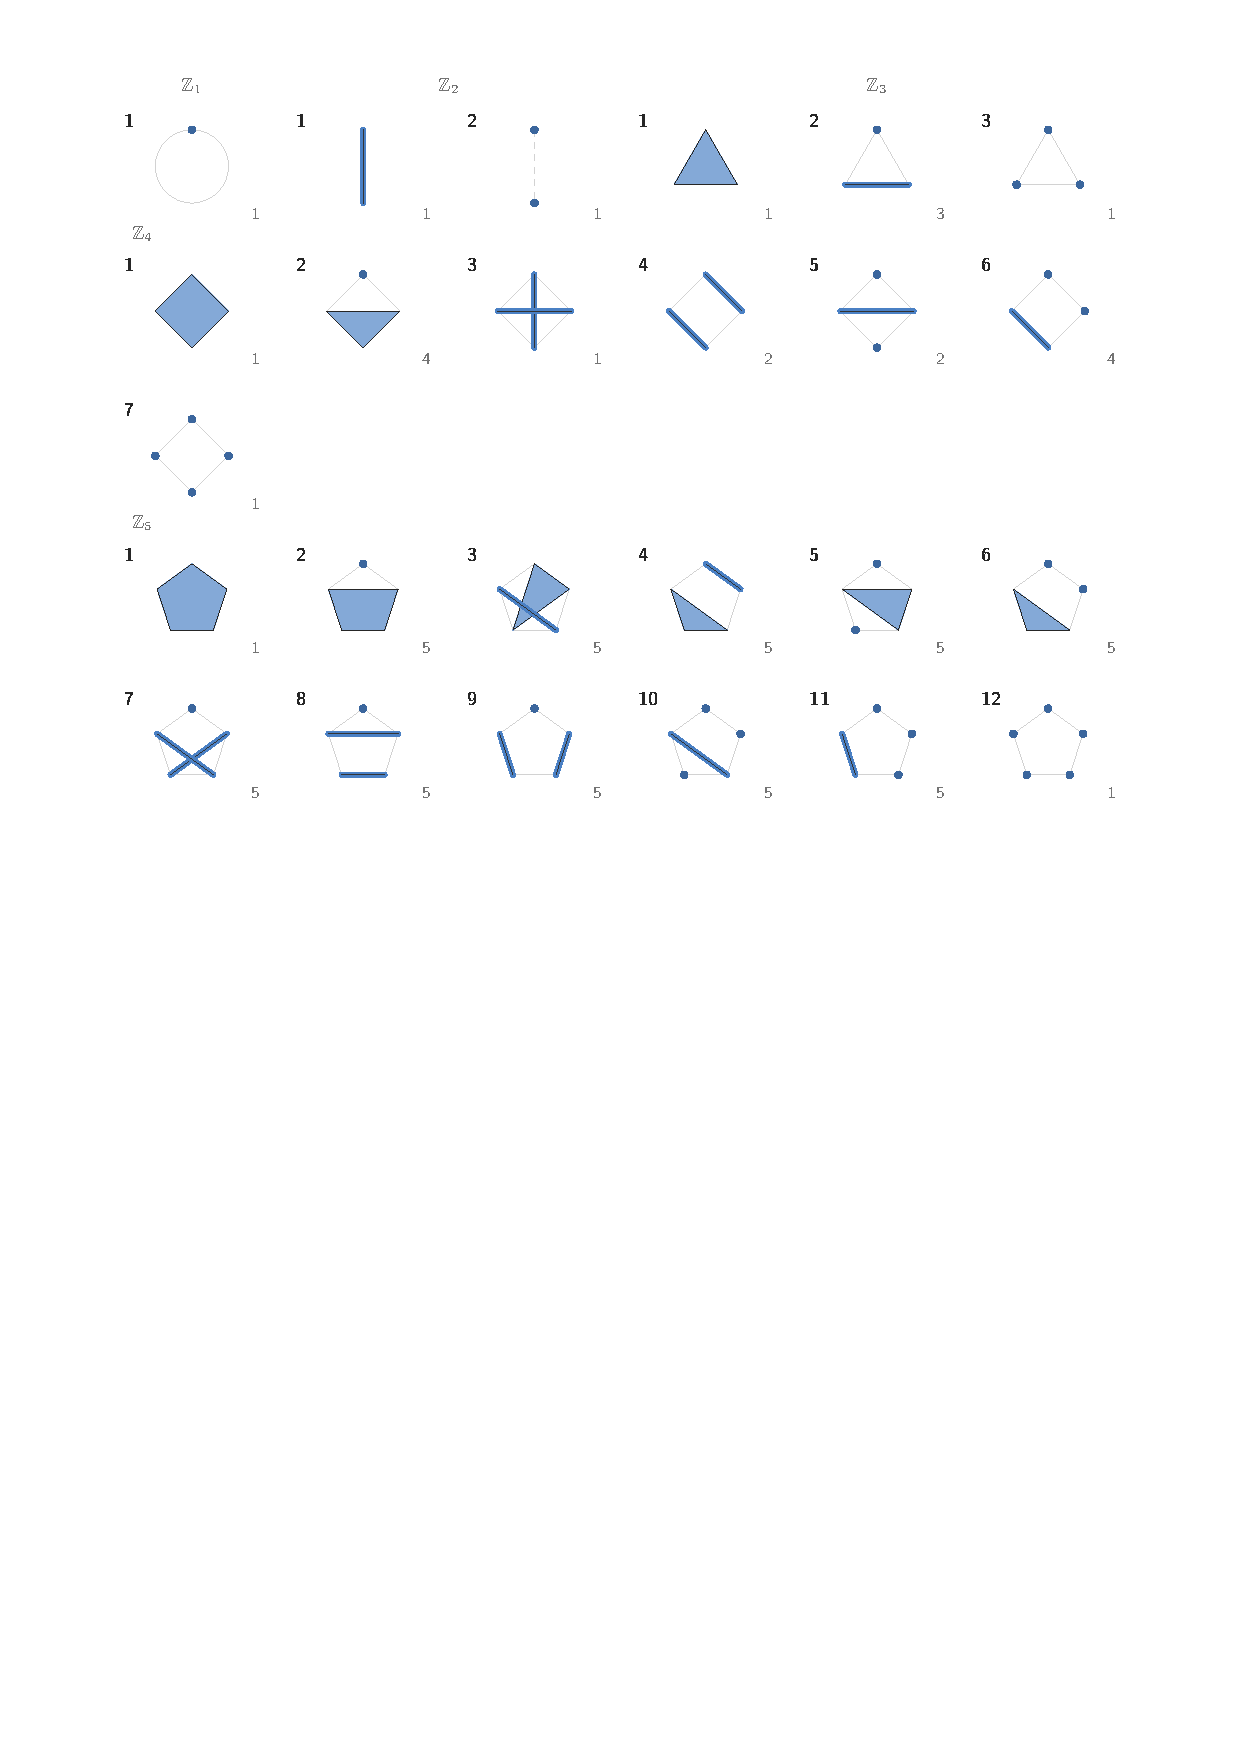
\includepdf[pages=1, offset=0 -16mm, pagecommand={\thispagestyle{headings}}]{plates/plates_z1_z8.pdf}
\phantomsection
\label{plate:2}
\includepdf[pages=2, offset=0 -16mm, pagecommand={\thispagestyle{headings}}]{plates/plates_z1_z8.pdf}
\phantomsection
\label{plate:3}
\includepdf[pages=3, offset=0 -16mm, pagecommand={\thispagestyle{headings}}]{plates/plates_z1_z8.pdf}
\phantomsection
\label{plate:4}
\includepdf[pages=4, offset=0 -16mm, pagecommand={\thispagestyle{headings}}]{plates/plates_z1_z8.pdf}
\phantomsection
\label{plate:5}
\includepdf[pages=5, offset=0 -16mm, pagecommand={\thispagestyle{headings}}]{plates/plates_z1_z8.pdf}
\phantomsection
\label{plate:6}
\includepdf[pages=6, offset=0 -16mm, pagecommand={\thispagestyle{headings}}]{plates/plates_z1_z8.pdf}
\phantomsection
\label{plate:7}
\includepdf[pages=7, offset=0 -16mm, pagecommand={\thispagestyle{headings}}]{plates/plates_z1_z8.pdf}
\phantomsection
\label{plate:8}
\includepdf[pages=8, offset=0 -16mm, pagecommand={\thispagestyle{headings}}]{plates/plates_z1_z8.pdf}
\phantomsection
\label{plate:9}
\includepdf[pages=9, offset=0 -16mm, pagecommand={\thispagestyle{headings}}]{plates/plates_z1_z8.pdf}
\phantomsection
\label{plate:10}
\includepdf[pages=10, offset=0 -16mm, pagecommand={\thispagestyle{headings}}]{plates/plates_z1_z8.pdf}


\backmatter
\bibliographystyle{plain}
\bibliography{octatlas}

\end{document}
